\documentclass[pagesize, paper=a4, fontsize=12pt,titlepage=true, headings=small, headnosepline, abstractoff, liststotoc, nochapterprefix, plainheadsepline, twoside]{scrreprt}
\usepackage[a4paper, left=40mm, right=30mm, top=20mm, bottom=30mm]{geometry}
\usepackage[utf8]{inputenc}
\usepackage[ngerman]{babel}
\usepackage[babel,german=guillemets]{csquotes}
\usepackage[backend=biber, style=apa]{biblatex}
\usepackage{amsmath}
\usepackage{amsfonts}
\usepackage{amssymb}
\usepackage{makeidx}
\usepackage{setspace}
\usepackage{color}
%\usepackage{cite} % Paket fuer die Zitation
% \usepackage{natbib} % Erweitertes paket für Zitate.
%\usepackage{sourcesanspro}
\usepackage[T1]{fontenc}
\usepackage{lmodern}
% Bilder Settings
\usepackage{graphicx}
\usepackage [singlelinecheck=false] {caption}
\usepackage{subcaption}
\usepackage{url}
\usepackage{scrpage2}
\usepackage [singlelinecheck=false] {caption}
\usepackage{pdfpages}


% Paket fuer das anzeigen von Sourcecode
\usepackage{listings}
% Setze die Programmiersprache auf CSharp
\lstset{language=[Sharp]C} 

% Festlegung Art der Zitierung -NatDin für Deutschland: Abkuerzung Autor + Jahr
%\bibliographystyle{jurabib}
\DeclareLanguageMapping{german}{german-apa}
\DefineBibliographyStrings{ngerman}{%
    bibliography={Literaturverzeichnis}% NICHT references
}
\addbibresource{Biblatex/VerzeichnisBuecher.bib}
%plain

% Festlegen der Sprache
\selectlanguage{ngerman}

% Settings fuer den Sourcecode START
\definecolor{mywhite}{rgb}{1,1,1}
\definecolor{mygreen}{rgb}{0,0.4,0}
\definecolor{mygray}{rgb}{0.5,0.5,0.5}
\definecolor{mykeywordgray}{rgb}{0.2,0.2,0.2}
\definecolor{mymauve}{rgb}{0.58,0,0.82}
\definecolor{bggray}{rgb}{0.97,0.97,0.97}
\definecolor{titlegray}{rgb}{0,0,0}
\definecolor{titleblack}{rgb}{0,0,0}

% Farbe für die Überschriften
%\addtokomafont{sectioning}{\color{titleblack}\rmfamily}

% URL Style
\urlstyle{rm}

\lstset{
backgroundcolor=\color{mywhite},  % choose the background color; you must add \usepackage{color} or \usepackage{xcolor}
basicstyle=\small, % the size of the fonts that are used for the code
breakatwhitespace=false,         % sets if automatic breaks should only happen at whitespace
breaklines=true,                 % sets automatic line breaking
captionpos=b,                    % sets the caption-position to bottom
commentstyle=\small\color{black},    % comment style
deletekeywords={...},            % if you want to delete keywords from the given language
escapeinside={\%*}{*)},          % if you want to add LaTeX within your code
extendedchars=true,              % lets you use non-ASCII characters; for 8-bits encodings only, does not work with UTF-8
frame=single,                    % adds a frame around the code
keepspaces=true,                 % keeps spaces in text, useful for keeping indentation of code (possibly needs columns=flexible)
keywordstyle=\color{mykeywordgray}\bfseries,       % keyword style
language=[Sharp]C,                 % the language of the code
morekeywords={*,Select,where,select,Write, from, in, orderby, IEnumerable, Where, OrderBy, FindIndex, List, Count, Insert, Remove},            % if you want to add more keywords to the set
numbers=left,                    % where to put the line-numbers; possible values are (none, left, right)
numbersep=10pt,                   % how far the line-numbers are from the code
numberstyle=\color{mykeywordgray}, % the style that is used for the line-numbers
rulecolor=\color{titlegray},         % if not set, the frame-color may be changed on line-breaks within not-black text (e.g. comments (green here))
showspaces=false,                % show spaces everywhere adding particular underscores; it overrides 'showstringspaces'
showstringspaces=false,          % underline spaces within strings only
showtabs=false,                  % show tabs within strings adding particular underscores
stepnumber=1,                    % the step between two line-numbers. If it's 1, each line will be numbered
stringstyle=\color{black},     % string literal style
tabsize=2,                       % sets default tabsize to 2 spaces
title=\lstname,                   % show the filename of files included with \lstinputlisting; also try caption instead of title
captionpos=t,
aboveskip=1\baselineskip,		% Platz über dem quellcode block
belowskip=1\baselineskip,			% Platz unter dem quellcode block
%morecomment=[il]{///}
}
% Settings fuer den Sourcecode ENDE

% Listings
\renewcommand{\lstlistlistingname}{Verzeichnis der Sourcecode Beispiele}
\renewcommand{\lstlistingname}{Sourcecode Beispiele}

% Autoren
\author{
Dominik Steffen \and
Erstbetreuer: Prof. Christoph Müller, Fakultät DM \and
Zweitbetreuer: Prof. Dr. Wolfgang Taube, Fakultät DM
}


% Titel
\title{Splitting Game Development Processes for Good}
\subtitle{Konzeption und Implementierung eines Beispielhaften Game Authoring Prozesses unter betrachtung von Game Engine Tool Development Aspekten .... TBD}
\parindent 0pt


%%%%%%%%%%%%%%%%%%%%%%%%%%%%%%%%%%%%%%%%%%%%%%%%%%%%%%%%%%%%%%%%%%%%%%%%%%%%%%%%
%	Commands START - Makros
%%%%%%%%%%%%%%%%%%%%%%%%%%%%%%%%%%%%%%%%%%%%%%%%%%%%%%%%%%%%%%%%%%%%%%%%%%%%%%%%
% C# makro OHNE space nach dem logo
\newcommand{\CS}{C\texttt{\#}}
% C# makro MIT space nach dem logo
\newcommand{\CSS}{C\texttt{\# }}
% C++ Logo
\newcommand{\CPP}{C\nolinebreak\hspace{-.05em}\raisebox{.4ex}{\tiny\bf +}\nolinebreak\hspace{-.10em}\raisebox{.4ex}{\tiny\bf +}}
% LINQ For Geometry
\newcommand{\LFG}{LINQ For Geometry}
% LINQ For Geometry mit Space
\newcommand{\LFGS}{LINQ For Geometry }
% LINQ mit spaces links und rechts
\newcommand{\LQ}{ LINQ }
% Generic zeichen <T>
\newcommand{\GT}{\textless T\textgreater}
\newcommand{\GTS}{\textless T\textgreater\space}
% Lambda Zeichen in C#
\newcommand{\LAM}{ =\textgreater\space}
% HES
\newcommand{\HES}{Half-Edge Datenstruktur }
%%%%%%%%%%%%%%%%%%%%%%%%%%%%%%%%%%%%%%%%%%%%%%%%%%%%%%%%%%%%%%%%%%%%%%%%%%%%%%%%
%	Commands ENDE
%%%%%%%%%%%%%%%%%%%%%%%%%%%%%%%%%%%%%%%%%%%%%%%%%%%%%%%%%%%%%%%%%%%%%%%%%%%%%%%%


%%%%%%%%%%%%%%%%%%%%%%%%%%%%%%%%%%%%%%%%%%%%%%%%%%%%%%%%%%%%%%%%%%%%%%%%%%%%%%%%
%	Unterstrichene Kapitelüberschriften START
%%%%%%%%%%%%%%%%%%%%%%%%%%%%%%%%%%%%%%%%%%%%%%%%%%%%%%%%%%%%%%%%%%%%%%%%%%%%%%%%
\newcommand*{\ORIGchapterheadendvskip}{}%
\let\ORIGchapterheadendvskip=\chapterheadendvskip
\renewcommand*{\chapterheadendvskip}{%
\ORIGchapterheadendvskip
{%
\setlength{\parskip}{0pt}%
\noindent\rule[3\baselineskip]{\linewidth}{1pt}\par
}%
}
%%%%%%%%%%%%%%%%%%%%%%%%%%%%%%%%%%%%%%%%%%%%%%%%%%%%%%%%%%%%%%%%%%%%%%%%%%%%%%%%
%	Unterstrichene Kapitelüberschriften ENDE
%%%%%%%%%%%%%%%%%%%%%%%%%%%%%%%%%%%%%%%%%%%%%%%%%%%%%%%%%%%%%%%%%%%%%%%%%%%%%%%%

\newpage

\makeindex
\onehalfspacing
%\setuptoc{toc}{numbered}

\begin{document}
% Titelblatt START
%\maketitle
%\addcontentsline{toc}{chapter}{Titelblatt}
\includepdf[pages={1}]{Includes/deckblatt.pdf}
% Titelblatt ENDE


%%%%%%%%%%%%%%%%%%%%%%%%%%%%%%%%%%%%%%%%%%%%%%%%%%%%%%%%%%%%%%%%%%%%%%%%%%%%%%%%
%	Abstract START
%%%%%%%%%%%%%%%%%%%%%%%%%%%%%%%%%%%%%%%%%%%%%%%%%%%%%%%%%%%%%%%%%%%%%%%%%%%%%%%%
\newpage
\thispagestyle{empty}
\mbox{}

\begingroup
\newpage
\pagestyle{empty}
\renewcommand*{\chapterpagestyle}{empty}
\chapter*{Abstract}%
%\addcontentsline{toc}{chapter}{Abstract}
Arbeitsprozesse in heutigen Game Engines verlangen von Entwicklern meist das erlernen neuer Toolsets und das während eines meist sehr eingeschhränkten Projekt Zeitraums. Es wäre für Entwickler einfacher sich mit den bereits bekannten Tools zu beschäftigen und mit diesen großartige Ergebnisse zu erreichen. Designer müssen sich oft in unbekannte Editoren und SDKs einarbeiten während Entwickler sich in Grafische Editoren einarbeiten sollen um ihren Code an der richtigen Stelle des Projekts einzubinden.
Diese Arbeit baut eine Brücke zwischen beiden Welten. Durch die Konzeption und Umsetzung eines Software Tools und Entwicklungsprozesses wird eine Trennung der Abhängigkeiten in einem Projekt erreicht. Mit Hilfe eines Plugins ist es möglich, dass Designer oder Entwickler jederzeit mit ihren eigenen Tools in die Entwicklung eines Projektes einsteigen. Es wird ermöglicht mit Cinema 4D und einer IDE wie VS2013 an einem Projekt mit der FUSEE Engine zu arbeiten ohne die bereits bekannte Welt zu verlassen. Ein FUSEE Projektstruktur "managed" sich durch die Nutzung des entstandenen Cinema 4D Plugins und den generierten Visual Studio Solution Dateien selbst.
Das zuerst konzeptionell entworfene Tool wurde während dieser Arbeit umgesetzt und bietet ausreichende Basisfunktionalität um ein Projekt als Entwickler als auch als Artist zu erstellen und zu bearbeiten. Hierzu wurden verschiedene Konzepte betrachetet und andere GameEngines auf Workflow und Anwendbarkeit untersucht. Es wurden einige Kernkonzepte erkannt und für eine Implementierung in FUSEE Uniplug analysiert und weiter entwickelt.
\clearpage
\endgroup
%%%%%%%%%%%%%%%%%%%%%%%%%%%%%%%%%%%%%%%%%%%%%%%%%%%%%%%%%%%%%%%%%%%%%%%%%%%%%%%%
%	Abstract ENDE
%%%%%%%%%%%%%%%%%%%%%%%%%%%%%%%%%%%%%%%%%%%%%%%%%%%%%%%%%%%%%%%%%%%%%%%%%%%%%%%%

%%%%%%%%%%%%%%%%%%%%%%%%%%%%%%%%%%%%%%%%%%%%%%%%%%%%%%%%%%%%%%%%%%%%%%%%%%%%%%%%
%	Versicherung START
%%%%%%%%%%%%%%%%%%%%%%%%%%%%%%%%%%%%%%%%%%%%%%%%%%%%%%%%%%%%%%%%%%%%%%%%%%%%%%%%
\newpage
\thispagestyle{empty}
\mbox{}

\begingroup
\pagestyle{empty}
\newpage
\renewcommand*{\chapterpagestyle}{empty}
\chapter*{Eidesstattliche Erkl"arung}%
%\addcontentsline{toc}{chapter}{Eidesstattliche Erkl"arung}
Ich erkläre hiermit an Eides statt, dass ich die vorliegende Masterthesis selbständig und ohne 
unzulässige fremde Hilfe angefertigt habe. Alle verwendeten Quellen und Hilfsmittel die sowohl zum schreiben dieser Arbeit als auch zum Entwickeln des dazugeh"origen Sourcecodes benutzt wurden, habe ich angegeben.

\vspace*{3cm}
\hspace*{\fill}\begin{tabular}{@{}l@{}}\hline
\makebox[9cm]{Dominik Steffen, K"ussaberg den \today}
\end{tabular}
\clearpage
\endgroup
%%%%%%%%%%%%%%%%%%%%%%%%%%%%%%%%%%%%%%%%%%%%%%%%%%%%%%%%%%%%%%%%%%%%%%%%%%%%%%%%
%	Versicherung ENDE
%%%%%%%%%%%%%%%%%%%%%%%%%%%%%%%%%%%%%%%%%%%%%%%%%%%%%%%%%%%%%%%%%%%%%%%%%%%%%%%%

%%%%%%%%%%%%%%%%%%%%%%%%%%%%%%%%%%%%%%%%%%%%%%%%%%%%%%%%%%%%%%%%%%%%%%%%%%%%%%%%
%	Logo START
%%%%%%%%%%%%%%%%%%%%%%%%%%%%%%%%%%%%%%%%%%%%%%%%%%%%%%%%%%%%%%%%%%%%%%%%%%%%%%%%
\newpage
\thispagestyle{empty}
\mbox{}

\begingroup
\newpage
\thispagestyle{empty}
\vspace*{8cm}
%\includegraphics[width=\linewidth]{Bilder/Logo}
\vspace*{1cm}
\begin{quote}
"Hier steht ein wichtiges Zitat zur Entstehung dieser Arbeit."
\end{quote} - TBD.
\vspace*{5cm}

Dominik Steffen\\
Matr.-Nr.: 245857\\
Hochschule Furtwangen\\

E-Mail:\\
dominik.steffen@hs-furtwangen.de\\
dominik.steffen@gmail.com\\
\endgroup
%%%%%%%%%%%%%%%%%%%%%%%%%%%%%%%%%%%%%%%%%%%%%%%%%%%%%%%%%%%%%%%%%%%%%%%%%%%%%%%%
%	Logo START
%%%%%%%%%%%%%%%%%%%%%%%%%%%%%%%%%%%%%%%%%%%%%%%%%%%%%%%%%%%%%%%%%%%%%%%%%%%%%%%%
\newpage
\thispagestyle{empty}
\mbox{}

% Inhaltsverzeichnis START
\begingroup
	\clearpage
	\pagestyle{empty}
	%\addcontentsline{toc}{chapter}{Inhaltsverzeichnis} 
	\tableofcontents
	\clearpage
\endgroup
% Inhaltsverzeichnis ENDE
\newpage
\thispagestyle{empty}
\mbox{}

%%%%%%%%%%%%%%%%%%%%%%%%%%%%%%%%%%%%%%%%%%%%%%%%%%%%%%%%%%%%%%%%%%%%%%%%%%%%%%%%
% Inhalt START
%%%%%%%%%%%%%%%%%%%%%%%%%%%%%%%%%%%%%%%%%%%%%%%%%%%%%%%%%%%%%%%%%%%%%%%%%%%%%%%%

% Passe Seitenzahlen wieder an START
\renewcommand*{\chapterpagestyle}{plain}
\pagestyle{plain}
\setcounter{page}{0}
% Passe Seitenzahlen wieder an ENDE

%%%%%%
%	Einführung / Einleitung START
%%%%%%
\chapter{Anforderungen, Ziele und eine Fragestellung}
Arbeitsprozesse in heutigen Game Engines verlangen von Entwicklern meist das erlernen neuer Toolsets und dies während eines meist sehr eingeschhränkten Projekt Zeitraums. Es wäre für Entwickler einfacher sich mit den bereits bekannten Tools zu beschäftigen und mit diesen großartige Ergebnisse zu erreichen. Authoring Tools ermöglichen  also auch Teammitgliedern ohne weiteres tiefegend technisches Verständnis für die Programmierung von Spielen, an Projekten in der Entwicklung mitzuarbeiten.

\begin{quote}
It [Developing “Authoring Tools”, Anmerkung des Autors] is successful due to several factors: it allows non-technical users to work on projects that would otherwise be out of their reach (due to lack of expertise, especially concerning programming languages); it can bring struc-ture into unstructured domains (such as game development) and it can speed up de-velopment by streamlining and automating common tasks. \cite {FutureTrendsGAT:2012}
\end{quote}

\section{Motivation}
Diese Arbeit beschäftigt sich nun mit der Frage ob es möglich ist ein Tool zu konzipieren welches auf der Basis eines bereits bestehenden Modeling Editors (hier Cinema 4D von Maxon \footfullcite{MaxonC4d2014}) das Erstellen einer “fertigen”\footnote{Build fähige Version einer im Fusee Szenenformat abgespeicherten 3D Szene.} Szene für die 3D Engine Fusee\footnote{FUSEE (Furtwangen Simulationd and Entertainment Engine - \url{http://www.fusee3d.org})} ermöglicht. Hierbei wird nach der Konzeption versucht die Basis Funktionalität in Visual Studio mit Hilfe von \CSS Code und der nach \CSS gewrappten\footnote{Eine Software welche von einem anderen Stück software umgeben wird.} Cinema 4D API zu implementieren. Die gewrappte Cinema 4D API basiert auf einem ehemaligen Projekt der Hochschule Furtwangen. Dieses wird als Grundlage für die hier angedachte Implementierung genutzt und bietet einen geringen Umfang an Basisfunktionalität. So bietet es die Möglichkeit grundsätzlich Plugins für Cinema 4D in der Programmiersprache \CSS zu schreiben. Von Haus aus ermöglicht Maxon das Entwickeln von Plugins nur in C++, Python und Coffee (einer von Maxon selbst entwickelten Skriptsprache). Der Vollständigkeit halber sei gesagt, dass Maxon für C++ noch das Framework Melange anbietet welches es ermöglicht Cinema 4D Dateien ohne eine Cinema 4D installation zu erstellen, zu speichern und zu laden. Sollte eine Installation vorhanden sein kann das Plugin auch Szenen rendern.

Szenen in Cinema 4D werden grundsätzlich in einer Art Baumstruktur gespeichert und zur weiteren Verarbeitung im Speicher gehalten. Die hier konzipierte Software möchte diese Tatsache nutzen um Szenen aus einem Modeling Editor (Cinema 4D) in eine Szene des Fusee Szenen Formats (.fus) umzuwandeln. Eine “.fus” Datei ist ebenfalls in einer Baumartigen Struktur gespeichert. Dieses Prinzip der Szenendarstellung ist bereits aus verschiedenen Frameworks und Softwareprojekten für 2D Darstellung bekannt. Das ist zum einen der Übersichtlichkeit als auch verschiedenen Algorithmischen Operationen auf den Daten der Szene geschuldet. In Baumstrukturen organisierte Interfaces werden außerdem bei der Entwicklung des User Interfaces für das Mobile Betriebssystem Android verwendet.

\section{Ziele der Implementierung}
Die während dieser Arbeit implementierte Software hat das Ziel eine Basis für die Verwendung von Cinema 4D als Game Engine Editor aufzubauen. Es werden grundlegende Funktionen in Form einer \CSS Bibliothek entwickelt die es ermöglichen sollen das Projekt in Zukungt auch für andere 3D Modeling Software anzupassen. Diese Arbeit zielt nicht darauf ab ein komplettes Tool für die Entwicklung von Spielen in der Fusee Engine zu erschaffen. Es wird versucht eine art Grundstein für weitere Forschung und Entwicklung in den Bereich des Game Authoring Toolkit Developments für die Arbeit mit der Akademischen Simulations und Entertainment Software FUSEE zu legen. Das Kernziel ist das Erstellen eines Konzeptes und die Erläuterung der einzelnen Module eines solchen Systems. Verschiedene bereits bestehende Tools und Game Engines werden zu vergleichen herangezogen und wurden im Laufe dieser Arbeit untersucht und getestet.
\section{Verwendete Software}
\begin{itemize}
\item Microsoft Visual Studio 2010, \newline verwendet als Entwicklungsumgebung f"ur das Softwareprojekt.
\item Die Erweiterung ReSharper in Version 7.1 f"ur Visual Studio 2010 \url{http://www.jetbrains.com/resharper}
\item Umlet \url{http://www.umlet.com/} \newline Ein kostenloses Tool um UML Diagramme zu erstellen.
\item GitHub und die GitShell \url{www.github.com} \newline Verwendet als Versionskontrollsystem und als Distributionswerkzeug für den Sourcecode.
\item TexWorks \url{www.tug.org/texworks/} \newline Zum Schreiben dieser Arbeit.
\end{itemize}

\chapter{Grundlegendes}
\section{Entwicklungsprozesse in Interaktiver 3D Software und Games}
Um einen Entwicklungsprozess abzubilden und Tools für Entwickler, sogenannte Developer Tools, zu entwickeln bedarf es einer gewissen Organisation. Im Bereich der modernen Spieleentwicklung in kleinen bis mittleren Unternehmen (seltener bei großen AAA Produktionen \footnote{Allgemein: Hochqualitative Spiele Software mit großem Entwicklungsbudget und einer Breiten Zielgruppe. Vgl. \cite{GamasutraAAA2005} }) wird hierfür ein agiles Modell zur Softwareentwicklung eingesetzt. Hier soll ein kurzer Überblick über aktuelle Modelle entstehen. Diese Modelle ermöglichen zum einen das schnelle Entwickeln von Tools während der knappen Entwicklungszeit eines Spiele Produkts und zum anderen unterstützen sie die Arbeit von kleinen Teams, in welchen meist Tool Developement betrieben wird,  innerhalb eines großen Entwicklerteams um so gezielt plötzlich auftauchende Aufgaben ohne lange Planung und viel Bürokratie lösen zu können. Damit ist ein fortschreiten des gesamten Projektablaufs gesichert und Entwickler können ihre Zeit hauptsächlich für die Entwicklung der Tools investieren.
\subsection{Projektmanagement Modelle}
% Warhorse Scrum, Waterfall, etc.
Um große Projekte wie Computergames oder Interaktive Software zu entwickeln, bedarf es meist einer detaillierten Planung und einer exakten Rollenverteilung im Entwicklerteam. Es existieren verschiedene Methoden des Projektmanagement auf welche hier kurz im Zusammenhang mit der Arbeit eingegangen werden soll. Einige der Projektmanagement Modelle wirken auf die Arbeitsweise der Teammitglieder aus. Daher wird diese Arbeit hier keinen Umfassenden Überblick über Projektmangament Methoden geben, sondern nur solche Ansprechen die sich direkt oder indirekt stark auf das Tool Development auswirken.
\subsubsection{Agile Modelle vs. klassische Modelle}
Viele Entwickler (Ubisoft, siehe \cite{MKG:Schmitz2014}) setzen heute auf moderne Modelle zum Entwickeln von Software. Die so genannten agilen Modelle (wie Beispielsweise Scrum,  Extreme Programming und Feature Driven Development) ermöglichen meist das schnelle (agile) reagieren auf plötzlich auftauchende schwierige Situationen. Klassische Modelle (Wasserfallmodell, Spiralmodell) haben hier meist Probleme durch ungleich höhere Bürokratie und Komplexität und benötigen ein Zeitaufwändigeres re-iterieren im Falle von Updates und Umstrukturierungen in Folge von unvorhergesehenen Ereignissen und Problemen. Hochkomplexe Software Projekte die über längere Zeiträume entwickelt werden können meist nur durch klassiche Projektmanagement Modelle überblickt und erfasst werden. Allerdings bedeutet der zusätzliche Bürokratische Mehraufwand auch oftmals einen erhöhten Overhead im Personal-, Software- und Knowledge-Bereich. Es ist im Fall des schnell-lebigen Tool Developments also geschickter, sich mit einem ebenso schnell-lebigen und agilen Projektmanagementmodell wie Scrum zu organisieren.
\subsubsection{Scrum}
Der Scrum Prozess tauchte das erste mal in der Veröffentlichung “The New New Product Development Game” von Hirotaka Takeuchi and Ikujiro Nonaka 1986 auf - damals nicht unbedingt in der Software- sondern der allgemeinen Produktentwicklung eingesetzt. Seitdem hat sich das Modell weiter entwickelt und erfreut sich bei innovativen Softareprojekten im Games und Indie-Games Bereich (auch und meist wohl auch vor allem im Tool Development) sehr großer Beliebtheit. Die Entwickler CCP und Warhorse Studios hatten hierzu eigene Videos und Artikel veröffentlicht, siehe \cite{CCP:ScrumAndAgile2009}, \cite{WH:Scrum2013}, \cite{WH:ScrumVideo2013}.

Ein Scrum Entwicklerteam ist mit folgenden Rollen besetzt:
\begin{itemize}
\item Product Owner
\item Entwicklungsteam
\item Scrum Master
\end{itemize}

Bei diesen Rollen handelt es sich um das interne Scrum Team - das Entwicklungsteam des Produktes. Scrum kann innerhalb eines Projektes und Teams beliebig heruntergebrochen werden, bis die gewünschte größe eines Entwicklerteams erreicht wird. Externe Rollen wie Stakeholder etc. verlagern sich somit auf andere interne Projektleiter oder Teammitglieder. Aus diesem Grund ist das Model gut für die Entwicklung von Development Tools und Toolkits geeignet. Mit Hilfe des Models, können benötigte Toolkits während einer Projektlaufzeit schnell und effizient entwickelt werden ohne dass ein schwerfälliger Bürokratischer Prozess die Entwicklung blockiert. Somit ergänzt sich dieser Prozess gut mit dem doch eher agilen entwickeln von Developement Tools während der Projektlaufzeit - denn in den seltensten Fällen wurde vor dem Beginn des Projekts daran gedacht alle nötigen Tools bereitzustellen. Oftmals ergeben sich auch während der Entwicklung neue Herausforderungen für das Team welche nach neuen Tools verlangen.

Hier soll nurn kurz ein Szenario aufgebaut werden, welches das Tool Developement Team eines aktiven Software Entwicklers beschreibt. Zuerst einmal sollen die Rollen verteilt werden:

\begin{itemize}
\item Product Owner - Meist der leitende Entwickler des Software Projektes. In diesem Fall meist ein Producer und/oder Game Developer.
\item Entwicklungsteam - Das Tool Development Team selbst.
\item Scrum Master - Die leitende Person des Tool Development Teams, bzw. sollte sich das Team sehr nah am Scrum Modell bewegen, dann meist ein Entwickler außerhalb des Teams aber mit guten Kontakten zum Team selbst und erhöhter Erreichbarkeit.
\end{itemize}

Die Stakeholder des Tools wären in diesem Fall die anderen Entwickler des Unternehmens die das Produkt im Produktiefbetrieb einsetzen möchten. Es kann hierbei auch von Vorteil sein, das Tool iterativ in den Arbeitsalltag des Teams zu integrieren um die Entwickler nicht durch einen Berg an neuen Features zu verunsichern und so die Einarbeitungszeit möglichst gering zu halten.
\\
\\
Es soll hier an einem kurzen Beispiel deutlich gemacht werden, wie ein solches Tool eingeführt werden könnte:
\\
\\
\textbf{Szenario}: Ein Team benötigt einen Textur-Editor / Tool um Texturen in das Format der Game-Engine zu transformieren.
\begin{itemize}
\item Der Antrag für das Tool vom Producer/Entwickler/oder anderen Personen wird gestellt.
\item Das Tool wird bewilligt und das Tool Development Team wird beauftragt.
\item Das Team entwickelt designed das Tool und implementiert Basisfunktionalität.
\item Das Tool wird mit der Basisfunktionalität an das Produkt Team herausgegeben.
\item Die fehlenden Funktionen werden implementiert.
\item Das Tool wird mit der erweiterten Funktionalität herausgegeben.
\item Es wird mit dem Produkt Team Rücksprache gehalten, welche Funktionen noch benötigt werden.
\end{itemize}
Dieser Prozess schließt iterrativ ab bzw. nicht ab, da während der Entwicklung einer interaktiven Anwendung / Games eventuell auch auf externe Einflüsse wie Third Party Software oder Marktentwicklungen eingegangen wird. Als Beispiel: So könnte sich durch die Veröffentlichung einer neuen GPU Generation oder den vorgezogenen PC Release die Größe der benötigten Textur-Dateien ändern.

\subsection{Internes Tool Developing oder Tool licencing}
Internes Tool Development ist ein wichtiger Aspekt im Team eines Games und Software Entwicklerteams. Erich Bethke berichtet  in davon, dass Michael Abrash\footnote{Ehemals idSoftware, ehemals Valve VR, aktuell Chief Scientist bei Oculus \url{https://www.oculus.com/company/}} ihm einst mitteilte, “dass 50\% der Entwickler Arbeit bei idSoftware in das Tool Development fliesse.” vgl. \fullcite[S. 44]{Bethke2003}.An der Relevanz des Themas hat sich trotz des zurückliegenden Zeitraums kaum etwas getan. Sony hat für den Release der Playstation 4\footnote{Playstation 4 - Erschienen im Herbst 2013} ein Development Kit \footfullcite{DVLP:Freeman2014} für die internen Entwickler Studios  erstellen lassen, welches bereits während der Planung und Entwicklung der Konsole entwickelt wurde. Sony hat diese Prozedur perfektioniert und lässt die eigenen Tools sogar in einem eigens dafür gegründeten Unternehmen für die eigenen Studios erstellen \footnote{SNSystems \url{http://www.snsystems.com/}}. Sony hat im Herbst 2014 den für Playstation 3 Spiele eigens intern entwickelten Welt Editor “Level Editor”\footfullcite{GS:SonyLE2014} als Open Source Software veröffentlicht und für Jedermann auf GitHub verfügbar gemacht. Der Editor kommt ohne direkten Enginebezug aus und lässt sich somit für verschiedenste Projekte der Sony Studios anpassen. Das ATF Framework, auf welchem viele interne Tools von Sony basieren\footnote{Hier ein Einführungsvideo: \url{https://www.youtube.com/watch?v=aU-9vzFELxc}}, kann von Sound Editoren über Cinematic Editoren bis hin zu State Machine Visualisierungen genutzt werden.Eine Übersicht vonn Tools, welche das ATF Framework erfolgreich verwendet haben findet sich unter \url{https://github.com/SonyWWS/ATF/wiki/ATF-Gallery}. Natürlich ist hier trotzdem noch ein gewisser grad an Aufwand zu betreiben, aber durch das integrierte ATF Framework werden viele Bereiche mit wiederverwendbarem Code abgedeckt. Sony Hauseigene  Entwicklerstudios haben ebenfalls ihre eigenen Tool Kits und Editoren auf dem von Sony bereitgestellten ATF Framework und “Level Editor” erstellt um Spiele wie Naughty Dogs Uncharted\footfullcite{NaughtyDog2007}, Guerilla Games’ Killzone Serie\footfullcite{GuerillaGames2004} oder Quantic Dreams Beyond:Two Souls\footfullcite{QuanticDream2013} zu erstellen. Eine Übersicht der Studios welche das ATF Framework verwenden findet sich unter dieser Adresse \url{https://github.com/SonyWWS/ATF/wiki/ATF-Adoption}. Dieser große Einfluss des Frameworks zeigt, dass selbst in großen - und kleineren - Studios immernoch Bedarf nach einfach und schnell zu erweiternden Frameworks und Editoren besteht. Das ATF Framework bzw. der “Level Editor” von Sony waren auch ein Anlass das das praktische Projekt zu dieser Arbeit an zu implementieren.

% TODO https://github.com/SonyWWS/ATF/wiki/High-Level-View-of-ATF
% Eventuell könnte hier noch interessanter Inhalt dazu kommen.

% MEF: runtime extensibility problem solution - kurz also plugin module.

\section{Mitglieder eines Entwicklerteams}
Es soll hier ein kurzer Überblick über die gängigsten Mitglieder eines Entwicklerteams gegeben werden. Grob können Entwickler in die folgenden drei Gruppen aufgeteilt werden - Artist, Designer, Engineer. Jede Gruppe arbeitet hierbei meist interdisziplinär mit den anderen zusammen, kümmert sich aber doch um die ganz eigenen Bestandteile eines Produktes. Es ist durchaus so, dass jede Gruppe ihre eigenen Tools und Methoden verwendet. Dieser Ansatz wird in der Konzeptionierung dieser Arbeit aufgegriffen und weiter verfolgt.

Bei der Bezeichnung und Aufteilung der verschiedenen Teammitglieder in Fachbereiche orientiert sich diese Arbeit am Werk von \fullcite{Chandler2006}, in welchem er die Produktionsprozesse eines Spiels sowohl in designtechnischer Weise als auch aus technischer Sicht beschreibt.

\subsection{Artists}
Artists sind in einem Games Projekt für jegliche Repräsentation der Spiellogik nach Außen zuständig. Sie erstellen Modelle von Spielfiguren und Umgebungen und kreiiren Texturen und User Interfaces. Bei den Artists handelt es sich um eine Kerngruppe für diese Arbeit da sie einen Großteil der Arbeitszeit in den Tools und Editoren des Spiels verbringt. Artists können in mehrere Untergruppen aufgeteilt werden. Dies bedeutet jedoch nicht, dass jedes Unternehmen jede Artists Rolle beschäftigt. Oftmals übernehmen einzelne Mitarbeiter mehrere Rollen je nach dem Entwicklungsstand des Projekts.
\subsubsection{Modeling/Animation Artist}
Ein Animation Artist verbringt die meiste Zeit damit Animationen und Modelle (3D, 2D), kurz: Assets \footnote{Assets sind Bestandteile des Produktes welche eine Grafische oder logische Repräsentation im Produkt erfahren. Dazu zählen z.B. Modelle, Texturen und Code Dateien.}, für die Verwendung im Spiel vorzubereiten. Programme wie Cinema 4D\footcite{MaxonC4d2014}, 3DS Max \footcite{AutodeskMax2014}, oder Modo\footcite{FoundryModo2014} sind Beispiele für Kernsoftware dieser Entwickler. Der vollständigkeit halber sei hier noch das Open Source Projekt Blender \footcite{Blender2015} erwähnt.

\subsubsection{Environment Artist}

\subsection{Designer}
Designer (Gamedesigner) arbeiten eng mit Artists und Engineers zusammen. Meist Entwicklen Game Designer das Spielprinzip, den Raum des Spiels und das Regelwerk. Sie schreiben oft Skripte und kleine Implementierungen oder verbessern Grafiken oder Spielfunktionen. Sie verwenden Assets aus der Designabteilung und fügen diese mit Skripten zusammen. Spieltests werden von Ihnen überwacht um den Spielfluss und das Erlebnis des Rezipienten beim Spielen zu optimieren.
\subsubsection{Level/World Designer}
Level bzw. World Designer erstellen aus den erschaffenen Assets eine oder mehrere zusammenhängende Spielwelten - sogenannte Level. Diese Welten werden durch sie und weitere Artists mit Inhalt nach den Plänen der Game Designer gefüllt. Oft haben diese Welten einen gewissen gestalterischen Anspruch und von den Designern erwünschten Artstyle welche die Atmosphähre des Spiels repräsentiert. Meistens werden diese Welten in einem extra dafür geschaffenen Editor angefertigt und können nich in einem Modeling Tool wie Cinema 4D entwickelt werden. Ein Beispiel für solche Level Editoren ist der GTKRadiant\footnote{Open Source Projekt GTKRadiant http://icculus.org/gtkradiant/} Editor für Spiele basierend auf der idTech3 und idTech4  Engine \footnote{Beide Engines und weiterer Source Code von idSoftare herunterzuladen auf dem Account des Unternehmens auf GitHub unter \url{https://github.com/id-Software} - geprüft am 08.04.2015}, beide als Open Source auf der Platform GitHub verfügbar. Weitere Beispiele sind der Level Editor von Sony, auf welchen diese Arbeit später noch eingeht sowie der Unity3d Editor. Der Unity3d beinhaltet eine gesamte Game Engine, jedoch wird direktes Modeling und das erstellen von Texturen von Grund auf nicht unterstützt. Alle Assets, außer primitiver Geometrischer Objekte wie Würfel und Kugeln etc. müssen in externen Programmen erstellt und importiert werden.

Die Konzeptionierung dieser Arbeit wird nurn die versuchen einen Ansatz zu entwickeln der es ermöglicht zumindest einen Teil der Level und Welteditor Tools zu beseitigen. Somit könnten Level und World Designer und Environment Artists ihre Arbeit in die bereits bekannten Modeling Tools verlagern und so eine verbesserte Projektivität erreichen.

\subsubsection{Scripter}
Scripter sind meist dafür Zuständig verschiedene Ereignisse in einer für die Game Engine extra entwickelten Script Sprache zu beschreiben und so die Welt des Spiels interaktiver zu gestalten. Diese Aufgaben unterstützen die Spiellogik oder aber beschreiben die Funktionen ganzer Systeme wie z.B. die eines Aufgabensystems (Quest Systems) welches dem Spieler während des Spiels mitteilt, was er in der Spieltwelt zu tun hat. Hier sind allerdings viele Bestandteile eines Spiels anzuordnen. Meist werden 

\subsubsection{User Interface Designer}
User Interface Designer kümmern sich um das Erstellen von grafischen Schnittstellen welche die Interaktion mit dem Benutzer ermöglichen. Hierfür verwenden sie oft Scriptsprachen wie Actionscript von Adobe (Zur programmierung von Adobe Flash Interfaces) oder gar fertige Middelware wie Scaleform \footcite{AutodeskScale2014} ein Cross Plattform UI Solution Tool\footnote{Ermöglicht das erstellen von 2D, 2.5D und 3D Ui Elementen. Wird z.B. von der Unreal Engine 4 verwendet.} von Autodesk. Diese Gruppe der Entwickler wird durch diese Arbeit nur sehr gering beeinflusst. In der Fusee Engine werden Interfaces über Code Dateien eingebunden und daher in externen Grafikprogrammen und Visual Studio angefertigt.

\subsection{Engineer}
Engineers / Ingenieure arbeiten meist am Kern der Applikation und schrieben den Source Code für die Anwendung, Engine, Netzwerkfunktionen, KI, und Tools. Diese Entwickler arbeiten hauptsächlich in einer IDE \footnote{Integrated Developement Environment} wie Visual Studio (auf welches sich das zu dieser Arbeit konzeptionierte Tool bezieht) oder XCode \footnote{X-Code ist nur für MacOSX erhältlich}. Der in der IDE geschriebene Code wird dann von den Engineers selbst oder von Game Designer in der Engine verwendet. Hierbei kann sich das Tätigkeitsfeld ausweiten bis hin zur Entwicklung von Gamelogic \footnote{Logik des Spiels, ermöglicht das interagieren etc. mit und in der Software}.
\subsubsection{Tool Engineer}
Diese Arbeit bezieht sich auf den Bereich des Tool Development. Hierbei entwickelt ein kleines Team - meist während oder vor der eigentlichen Arbeit an einem Projekt die Tools für die restlichen Entwickler des Projektes. Diese Tool Palette kann von Textureditoren bis hin zu kompletten Welteditoren fast alles vorstellbare enthalten. Verschiedene Studios haben eigene Tool Developer Teams, welche sich nur um diesen Bereich des Produktes kümmern. Diese Teams betreuen auch meist den Modding Support für ein fertiges veröffentlichtes Produkt. Beispiele für Modding Tools sind z.B. das RedKit von CDProject Red für das Spiel The Witcher 1 und 2, der LevelEditor von Sony der in einer Open Source Version vorliegt oder das Creation Kit von Bethesda Softworks welches einen Modding Support für die Spiele der The Elder Scrolls Reihe bereit stellt.
\subsubsection{Computer-Grahics Engineer}
Computer Graphics Engineers beschäftigen sich meist mit dem entwickeln der eigentlichen Engine. Oft sind Graphics Engineere aber auch an der Tool Entwicklung beteiligt. Gerade in kleineren Unternehmen könnten die eigentlichen Strukturen schnell aufbrechen um Synergien zu nutzen.

\subsection{Weitere für diese Arbeit nicht relevante Teammitglieder}
In diesem Abschnitt sollen noch die restlichen Mitglieder des Teams erwähnt werden, welche Tools nutzen aber meist nicht an der Entwicklung der selbigen beteiligt sind.
\begin{itemize}
\item Sound Engineer
\item Bla
\item Bla 
\item Bla 
\item Bla 
\end{itemize}

\section{Stakeholderanalyse intern}
Um herauszufinden, welche Entwicklergruppen eines Teams von neuen Development Tools im Bezug auf Fusee betroffen wären, wurde eine Analyse durchgeführt, um die Stakeholder innerhalb des Teams abzubilden. In der Praxis wäre für die Konzeption bzw. das Systemdesign eines neuen Tools der Besuch der von der Tool Entwicklung betroffenen Teammitglieder am Arbeitsplatz und das beobachten der jeweils verrichteten Aufgaben sehr aufschlussreich. Durch diese Methode könnten Probleme im Arbeitsablauf frühzeitig identifiziert, behoben und besonders wichtige Features rechtzeitig vor Beginn der Implementierung in Erfahrung gebracht und geplant werden.

Eine Bedarfsanalye und eine allgemeine Analyse der Aufgabengebiete der jeweiligen Entwickler sollte in das System Design bzw. das Requirements Engineering ebenfalls mit einfließen. Hierzu könnten interviews mit den Entwicklern geführt werden. Dies ist eine schnelle Methode welche sich gut mit einem agilen Prozess wie Scrum vereinbaren lässt.

\section{Ein Arbeitsprozess wird entwickelt}
\subsection{Game Authoring / Game Development}
Game Development beschreibt allgemein das entwickeln einer Interaktiven Software, meist eines Spiels. Hierbei spielt es keine Rolle ob die Software der puren Unterhaltung dient oder sich dem Genre des Serious Games zuordnen lässt. Auch weitere interaktive Anwendungen ohne Unterhaltungsfaktor können in diese Kategorie fallen. Die Produktionsabläufe ähneln sich stark. Im Gegensatz zum Tool Development hat das Game Development meist den Auftrag am Ende ein für den Consumer zugängliches Produkt zu schaffen. Das Tool Development beschäftigt sich in erster Linie mit dem Erstellen der Werkzeuge welche benötigt werden um das Consumerprodukt zu entwickeln.

Es ist aber in der Tat so, dass Tool Development auch auf dem Consumer Markt ankommen kann. Verschiedene Entwickler stellen in der Vergangenheit ihre Tools den Fans und Kunden zur Verfügung. Aus diesen Tools haben sich selbst schon wieder Produkte wie Modifikationen\footnote{auch Mods genannt, Verändern das eigentliche Spiel oder ersetzen es in Form einer “Total Conversion” gleich ganz durch neue, eigens entwickelte Inhalte}, Patches oder Erweiterungen entwickelt. Einige Beispiele sind die das Creation Kit von Bethesda Softworks und die daraus entstandenen zahlreichen Fan Modifikationen wie Nehrim oder Enderal des Mod Teams SureAI\footnote{Freies Modifikations Team. \url{http://www.sureai.net}}.

% TODO Chandler2006 zitieren.

\subsection{Tool Development}
% Nach Wihlidal ... Warum wurde oben geklärt, hier den Prozess erläutern.
% Möglichkeiten vorstellen.
% Beispiele geben.
Nach Wihlidals Auffasung \parencite{Wihlidal2006} unterscheidet sich die Planung eines Projektes zur Erstellung eines Developer Tools nicht sehr von der Planung zur allgemeinen Entwicklung von Software. Es gelten hier vier Planungsphasen die den Projektablauf kennzeichnen. Der erste Schritt wäre eine allgemeine Planung des Tools. Diese beinhaltet Funktionen und Umfang des Tools. Eine Beschreibung der Anforderungen bzw. der Ziele des Projektes wird mit den begünstigten Entwicklern abgesprochen.

Die zweite Phase beschreibt eine Bedarfsanalyse der Stakeholder. Es werden Arbeitsabläufe skizziert und mit den Beteiligten durchgesprochen. Je nach Komplexität und Relevanz des Projekts wird Software anderer Hersteller oder anderer Arbeitsbereiche ebenfalls analysiert und das Ergebnis zur Gesamtanalyse hinzugezogen. So könnte eventuell der Einsatz einer Drittanbieter Software in gewissen Situationen vorteilhafter sein als eine komplette interne Neuentwicklung. Diese Entscheidung ist aber sehr Situationsabhängig.

Daraufhin folgt die Designphase in welcher das Entwicklerteam des neuen Tools das Requirements Engineering abschliesst und mit dem Software-/Systemdesign beginnt. Hier wird das Produkt in Form von UML Diagrammen und Veranschaulichungen entwickelt. Die tatsächliche Implementierung folgt als letzte Phase des Projektablaufs. Während der Implementierung kann durch das agile Scrum System immer wieder iterativ an den Features des Tools gearbeitet werden.

Im folgenden Abschnitt wird noch etwas genauer auf die jeweiligen Schritte der Entwicklung eingegangen.

\subsubsection{Planung}
Es folgt die Planungsphase des Tools. Hier wird zuerst eine Requirementsanalyse \footnote{dt. Anforderungsmanagement} durchgeführt. Mit ihr sollen alle wichtigen Kerneigenschaften der Software identifiziert und niedergeschrieben werden. Ein an diese Arbeit angehängtes Designdokument führt diese Requirementsanalyse weiter aus. Die Anforderungsanalyse ist in einer solchen Situation, in welcher ein Produkt unter Zeitdruck für den Produktivbetrieb entwickelt wird, ein wichtiger Bestandteil der Projektplanung. Ein Tool, welches nicht den Anforderungen der Teammitglieder entpsricht kann nicht im Betrieb eingesetzt werden und verzögert im schlimmsten Fall die weitere Entwicklung des gesamten großen Softwareprojektes.

\subsubsection{Requirements Analyse}
\begin{itemize}
\item Eine Software soll es ermöglichen, dass Artists, Designer und Developer an ein und dem selben Projekt arbeiten können ohne die gewohnte Arbeitsumgebung (3D-Modellierungssoftware, IDE) zu verlassen und etwas komplett neues (Level-Editor) zu erlernen.
\item Das Produkt muss auf Basis der FUSEE Engine entstehen
\item Ziel ist es in Cinema 4D ein FUSEE Projekt anzulegen, zu speichern und es zu öffnen
\item Assets sollen ins Spiel integriert werden können die von Artists, Designern und Entwicklern bearbeitet werden können.
\item Das FUSEE \CSS Projekt sollte aus C4D heraus gebaut werden können.
%Hier könnte man einen Hinweis auf die Entwicklungsmethoden von id Software geben. Möglicherweise wäre eine Erwähnung der Pre-Rage Zeiten sinnvoll.
\item Eine Stakeholderanalyse schafft klarheit, welche Parteien des Teams mit dem zu erstellenden Tool arbeiten müssen.
\item Es ist zu analysieren, welche Schritte für welche Art der Arbeit des Teams notwendig sind. Hierzu werden Usecases der verschiedenen Rollen und Aufgaben erstellt.
\end{itemize}
\subsubsection{Requirements Dokumentation}
Während der Requirements Dokumentation werden alle Ansprüche an die Software Dokumentiert und von den Stakeholdern geprüft. Über dieses Dokument lässt sich der spätere Funktionsumfang des Tools genaustens definieren und verfolgen. Das Dokument stellt sozusagen ein rechtlich relevantes Dokument dar. Es findet sich im Anhang dieser Arbeit.

\subsubsection{System Design / System Modeling}
Anschließend an die Analyse folgt das System Modeling in welchem die Anforderungen des Programs zu einem Softwareprodukt modeliert werden. Oft bedient sich das Entwicklerteam hierbei Notationen wie UML \footnote{Unified Modeling Language} in Diagramm und Schrift Form. Das System Design ist ein kritischer Punkt. Hier müssen die Anforderungen des Kunden genau in die geplante Entwicklung des Systems übernommen werden. Oftmals arbeitet das System Design 

\subsubsection{Abgleich des System Designs mit den Anforderungen}
Vor der Implementierung muss immer auch geprüft werden ob das geplante System aus dem Designprozess mit den tatsächlichen Anforderungen der Stakeholder zusammen passt.

\subsubsection{Implementierung}
Die Implementierung ist der praktische Schritt des ganzen Prozesses. Während der Implementierung wird das Tool entwickelt, auf Fehler geprüft eventuell auch durch einen iterativen Entwicklungsprozess erweitert.

\subsubsection{Asset Pipeline und Feedback}
SEHR KRITISCHE MARKE! Das Asset aus dem Editor in die Engine bekommen, die Darstellung etc kontrollieren.
Zeitkritisch beim export etc.
Carter Seite 6 und folgende.
%Begriffserklärung eines Asset, genaue Definitionen anmerken.

\section{Die Struktur von Game Assets}
% TODO
Assets und das aufbrechen in Bestandteile eines Projektes. Level etc. bestehen aus Assets und mehr.
\subsection{Warum eine Trennung von Code und Content?}
%%%%%%
%	Einführung / Einleitung ENDE
%%%%%%

%%%%%%
%	Hauptteil START
%%%%%%
\chapter{Entwicklung eines Konzeptes}

% Planung
\section{Use Cases der verschiedenen Entwickler}
\subsection{Was möchten Artists?}
\subsection{Was möchten Designer?}
\subsection{Was möchten Entwickler?}

% Analyse
\subsection{Projekt bezogen}
\subsubsection{Projekt anlegen}
\subsubsection{Projekt öffnen}
\subsubsection{Projekt speichern}
\subsubsection{Projekt bauen}
\subsubsection{In Projekt einsteigen}
\subsubsection{Projekt clonen etc.}

\subsection{Prozess bezogen}
\subsubsection{Gleichzeitig an Projekt arbeiten}
\subsubsection{Model Datei importieren}
\subsubsection{Gleichzeitig an einem Objekt arbeiten}

\section{Aktuelle Engines und deren Arbeitsprozesse}
\subsection{Prozesse in Game Engines und einem Framework}
\subsection{Unreal Engine 4}
\subsection{Unity 3D}
\subsection{idTech X}
\subsection{Weitere}

% Design
\section{Konzeptentwurf}
\subsection{Systemdesign für ein Plugin}
\subsection{Systemdesign für einen Project-Handler}
\subsection{Entfernen von Abhängigkeiten}
\subsection{Zeitersparnis durch bekannte Tools}
\subsection{Warum Fusee und Cinema 4D?}

\begin{itemize}
\item Aufgrund der erstellten Use Cases und der Analysephasewird ein System Design erstellt. Meist eine UML basierte Darstellung.
\item Es soll möglichst wenig "geparsed" oder "konvertiert" werden
\item Dateien sollen Version Control kompatibel bleiben (wenig bis keine Binarys)
\item Das Projekt muss Strukturiert sein
\item Eine Fusee Solution soll gehandelt werden können
\end{itemize}

% Implementierung
\section{Die Implementierung}
Das Projekt “Fusee Authoring Toolkit” basiert auf mehreren Software Projekten. Ein Teil dieser Projekte wurde an der Hochschule Furtwangen entwickelt. Ein anderer Teil stammt von externen Entwicklen. Dieser Abschnitt gibt einen Überblick über die verwendeten Softwarebestandteile des Toolkits und ihrer Einbindung.

\subsection{Cinema 4D Plugin API und SDK}
Cinema 4D \autocite{MaxonC4d2014} ist ein kommerzielles proprietäres Produkt des Unternehmens MAXON Computer GmbH und steht nicht als Open Source Projekt zur Verfügung. Maxon stellt für die Entwicklung von Plugins\footnote{Plugins in C4D - Erweiterungen für die Software Cinema 4D und deren Funktionen} eine API\footnote{Application Programming Interface, z. Dt. Programmierschnittstelle} bereit. Bei dieser API handelt es sich um eine Bibliothek aus C++ Code. Dieser Code kann in Form von Header Files in die eigene Applikation integriert werden. Durch diese C++ Headerfiles ergibt sich eine Schnittstelle zu interenen Methoden in der Cinema 4D Software. Die tatsächlichen Methoden können mit der API nicht eingesehen werden, es handelt sich hier lediglich um Header Files ohne den Code der tatsächlichen Implementierung. Das C++ SDK wird bei einer Installation von Cinema 4D automatisch mitinstalliert. Auf einem Windows PC findet sich das SDK und die dazugehörigen Visual Studio Solution Dateien unter folgendem Pfad ausgehend vom Installations Ordner der 64Bit\footnote{Cinema 4D liegt seit der Version R15 nur noch als 64 Bit Version vor und benötigt laut \url{http://www.maxon.net/?id=311}(Maxon C4D System Requirements) ein 64 Bit System}: {“Cinema 4D/plugins/cinema4dsdk”}
\\
\\
Maxon stellt jegliche SDKs und Beispiele auf seinem GitHub Account unter der Apache License Version 2.0, January 2004\footnote{Apache Licence 2.0 \url{https://github.com/PluginCafe/cinema4d_cpp_sdk/blob/master/LICENSE}} zur freien Verfügung \url{https://github.com/PluginCafe}. Das C++ SDK ist unter dieser Adresse einsehbar: \url{https://github.com/PluginCafe/cinema4d_cpp_sdk}

Das folgende Schaubild erläutert die Verwendung der API. Es ist in der Tat som dass der eigene Plugin Code laut Maxons Dokumentation einige Funktionen überschreiben bzw. Klassen vererben muss. Ansonsten ist der Inhalt des Plugincodes nicht beschränkt. 

\begin{figure}[ht]
	\centering
  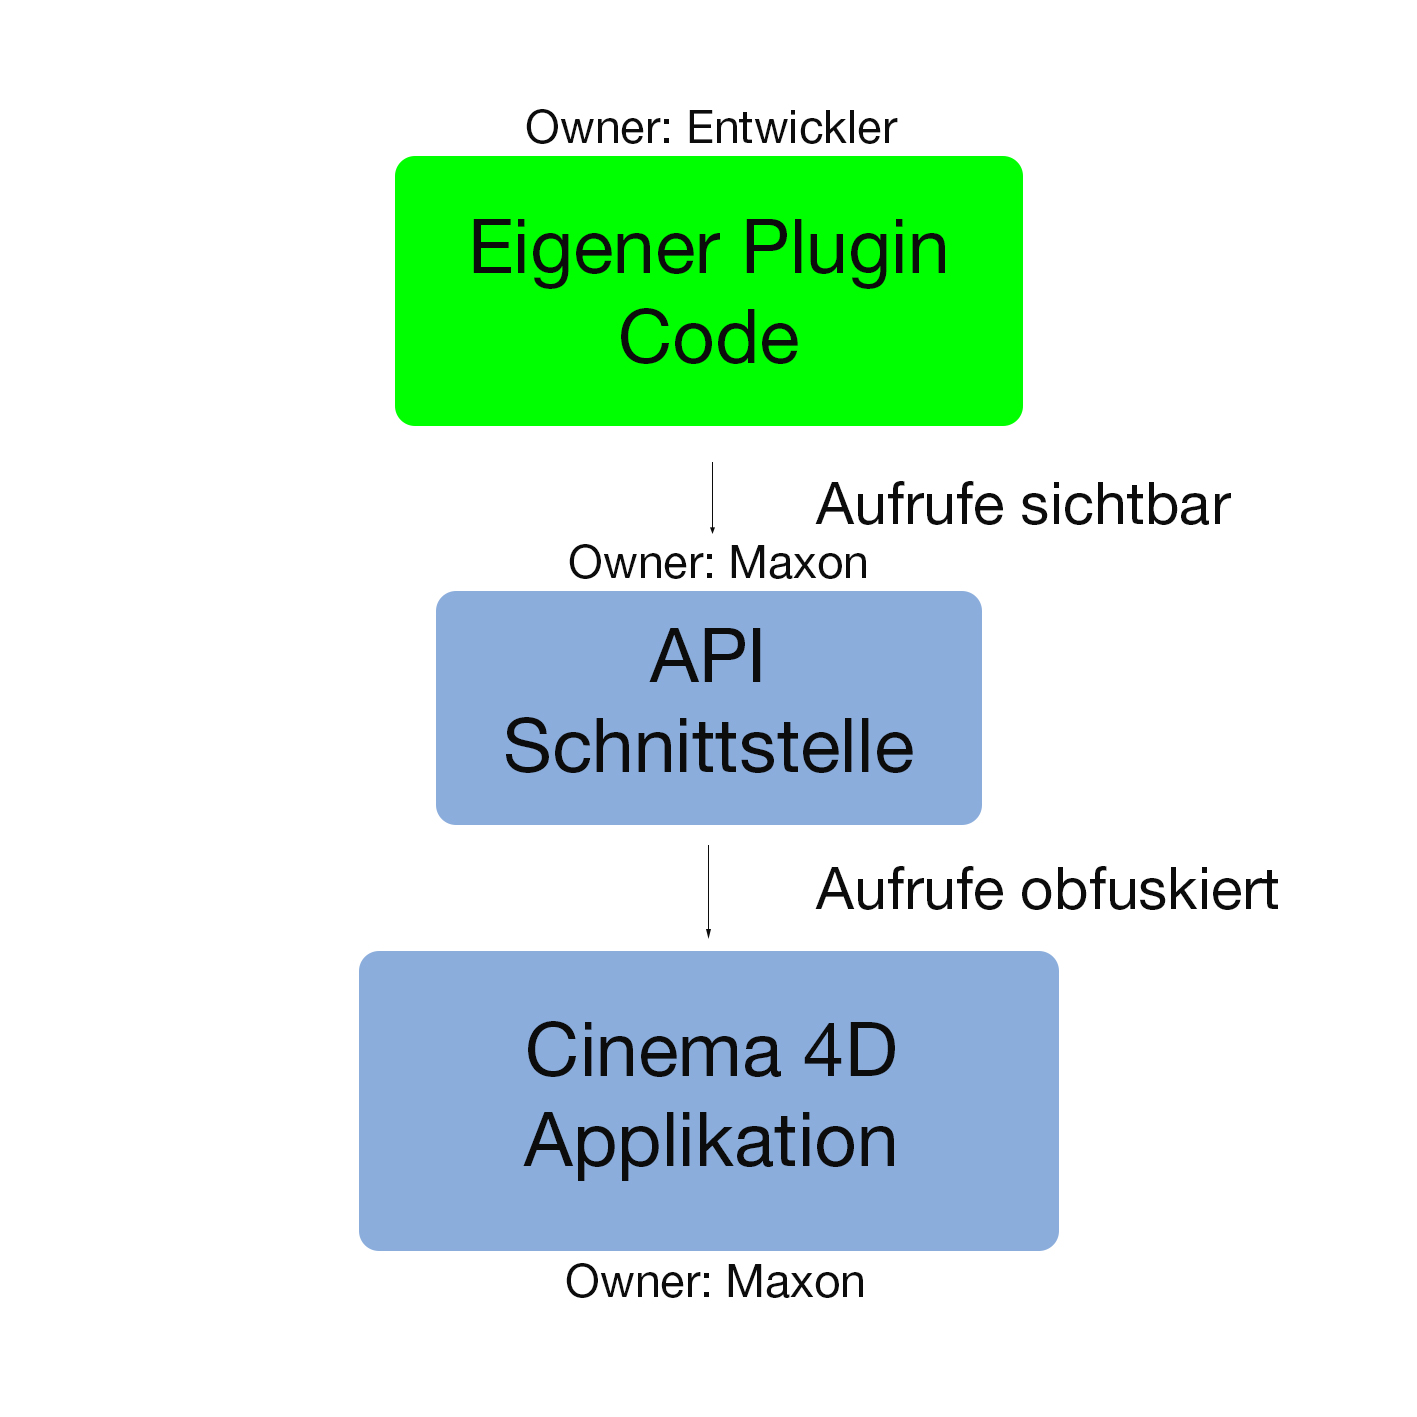
\includegraphics[width=\linewidth]{Bilder/C4D_Api_Schaubild_v1.jpg}
	\caption{Schaubild des Cinema 4D API Systems}
	\label{C4D API Schaubild}
\end{figure}

Das hier dargestellte Minimalbeispiel in C++ Code zeigt ein einfaches minimalistisches Plugin welches beim Ausführen nur eine Ausgabe auf der Konsole von Cinema 4D erzeugt.
\lstinputlisting[language=C++, caption = Einfaches Cinema 4D Plugin in der Programmiersprache C++]{Code/minimalbeispielPlugin.h}
Das hier dargestellte Code Beispiel wird im nächsten Abschnitt relevant. Es folgt ein Überblick über das Uniplug Projekt welches das Schreiben von Cinema 4D Plugins in \CSS ermöglicht. Die oben gezeigte  Codestruktur wird dann noch einmal als \CSS Version erläutert.

\subsection{Uniplug}
Bei Uniplug handelt es sich um ein Teil des Projektes FUSEE der Hochschule Furtwangen. Uniplug bietet die möglichkeit Cinema 4D Plugins in \CSS zu schreiben. Hierfür bedient es sich eines Interface Compilers SWIG\footnote{\url{http://www.swig.org/}}. Das gesamte Uniplug Projekt ist ein Open Source Projekt und steht im GitHub Repository unter \url{https://github.com/FUSEEProjectTeam/Fusee} innerhalb des Fusee Projekts zum Download bereit. Das Uniplug Projekt stand bereits vor dieser Arbeit zur Verfügung. Allerdings hatte es nich den nötigen Umfang und das Projekt wurde während der Arbeit um wichtige Funktionen zur Entwicklung von Plugins erweitert.
\subsubsection{Wrapping von C++ Code nach \CSS mit SWIG}
Um aus dem C++ Code der Cinema 4D API aufrufbaren \CSS Code zu erzeugen sind verschiedene Schritte notwendig. Ein SWIG Projekt welches im Uniplug Projekt verfügbar ist enthält eine C4dApi.i (interface) Datei. Diese Datei kümmert sich um das Wrappen des nativen C++ Codes nach \CS. Verschiedene Eintragungen die für das Erweitern des Uniplug Projektes vorgenommen wurden, werden im nächsten Abschnitt genauer erläutert.

Das hier abgebildete Schaubild zeigt den Ablauf des Wrapping-Vorgangs. Hierbei sind folgende Schritte zu erkennen:
\begin{itemize}
\item Erstellen des *.i Files und inkludieren der gewünschten nativen Code Dateien.
\item Überschreiben und/oder erweitern von nativen Code Dateien.
\item Kompilieren des SWIG Projektes.
\end{itemize}

% TODO
\begin{figure}[ht]
	\centering
%  \includegraphics[width=\linewidth]{Bilder/SWIG_Wrapping_v1.jpg}
	\caption{Wrapping Vorgang der Cinema 4D API von C++ nach \CS}
	\label{C4D API Schaubild}
\end{figure}

\subsubsection{Erweiterung des Uniplug Codes für Plugins vom Typ TagPlugin}
Um das Projekt auf den Aktuellen Stand zu bringen und das schreiben des Plugins zu ermöglichen musste zuerst das Uniplug Projekt erweitert werden. Auch hier wurde mit iterativen Methoden gearbeitet. Falls Probleme mit verschiedene Abhängigkeiten im C4D Api Code erkannt wurden, wurde zunächst geprüft, welche SWIG Dateien im \CSS API Code nicht vorhanden sind. Diese Dateien wurden dann inkludiert und es wurde versucht das SWIG Projekt zu bauen und die nun neu generierten und gewrappten \CSS Code Bestandteile im Plugin Code zu verwenden. In manchen Fällen war es nun nötig den nativen Code der API Dateien zu erweitern oder zu überschreiben. Bei der Implementierung des Cinema 4D Plugin Typs “TagPlugin” waren besondere Änderungen im API Code nötig. Hier sollen diese kurz aufgezeigt und erläutert werden.
\\
\begin{lstlisting}[language=C++, caption = Einbinden des Maxon Cinema 4D C++ Datentyps TagPlugin in die \CSS API von Uniplug]
#include "c4d_tagdata.h"
#include "c4d_tagplugin.h"

// "c4d_tagdata.h"
//%include "c4d_tagdata.h";
%feature("director") TagDataM;
%csmethodmodifiers TagDataM::TagDataM "private";
%typemap(cscode) TagDataM %{
	public TagDataM(bool memOwn) : this(C4dApiPINVOKE.new_TagDataM(), memOwn) {
    SwigDirectorConnect();
  }
%}
%include "c4d_tagdata.h";
%include "TagDataM.h";

// "c4d_tagplugin.h"
//%include "c4d_tagplugin.h";
%feature("director") TagPlugin;
%csmethodmodifiers TagPlugin::TagPlugin "private";
%typemap(cscode) TagPlugin %{
  public TagPlugin(bool memOwn) : this(C4dApiPINVOKE.new_TagPlugin(), memOwn) {
    SwigDirectorConnect();
  }
%}
%include "c4d_tagplugin.h";
\end{lstlisting}

Um den Datentyp TagData korrekt im \CSS Code zu verwenden, waren noch weitere Anpassungen im Code notwendig. Die Methode Message() des TagData ElternTyps NodeData musste Überschrieben werden im das Message System in \CSS nutzen zu können. Dies wurde nötig durch die Verwendung eines Void Pointers seitens Maxons in der Parameterliste der Message Funktion im C++ Code der API. SWIG kann an dieser Stelle durch den nicht auf einen Datentypen festgelegten Void Pointer des Datentyps der Parameterliste keine zufriedenstellende Wrappingfunktion bereit stellen. Das folgende Codebeispiel der Message() Funktion verdeutlicht den Fix im C++ Code des Uniplug Native Projektes.

Die Message() Funktion ist Teil des Nachrichtensystems innerhalb von Cinema4D. Viele Elemente des Programs und selbst geschrieben Plugins kommunizieren über dieses Messagesystem miteinander. Nachrichten von Cinema4D werden meist als Konstante Integer Variablen übergeben und können so in if else oder switch case Anweisungen vom Plugin Entwickler identifiziert und verarbeitet werden.

\begin{lstlisting}[language=C++, caption = Überschreiben der Message Funktion des TagData Datenty<ps.]
Bool TagDataM::Message(GeListNode *node, Int32 type, void *data)
{
	switch (type)
	{
	case MSG_EDIT:

		break;
	case MSG_GETCUSTOMICON:
		break;
	case COLORSYSTEM_HSVTAB:
		break;
	case MSG_DOCUMENTINFO:
		{
			DocumentInfoData* did = (DocumentInfoData*)data;
			return MessageDocumentInfo(node, did);
		}
		break;
	case MSG_DESCRIPTION_GETINLINEOBJECT:
		break;
	case DRAW_PARAMETER_OGL_PRIMITIVERESTARTINDEX:
		break;
	}

	return true;
}
\end{lstlisting}

Hier ist ersichtlich, dass die Funktion Message einen Void Pointer in der Parameterliste enthält. Dieser Voidpointer wird während der Funktion in andere Datentypen gecastet. Für die Wandlung der Message Funktion für die TagData Klasse war es von nöten ein Object des Typs DocumentInfoData zu erhalten. Aus diesem Grund, wird das Objekt dieses Typs bei einer bestimmten empfangenen Message ID zurück gegeben.

\subsubsection{Probleme}
Erst entwicklung von Uniplug erweitern bevor mit dem Plugin gearbeitet werden kann. Probleme durch das Wrappen und die fehlende Möglichkeit zu debuggen.

\subsection{Fusee}
\subsubsection{Der Fusee Szenengraph}
Das Fusee Level, Welt wie auch immer es hier bezeichnet werden sollte. Eine Basis wird gebraucht. Hierzu eine Zentrale anlaufstelle, ein Spiele “Kernel”? Irgend etwas dass im Zentrum steht.
Alles andere muss auf Level etc aufgeteilt werden und bis zum einzelnen Asset heruntergebrochen werden.

\section{Das eigentliche Plugin}
\subsection{Visualisierung der Systemarchitektur}
Schaubilder und Grafiken sind hier nützlich. Abhängigkeiten und Aufteilung sinnvoll gestalten.
\subsubsection{Welche Programme und Systeme sind beteiligt?}
Kette aufzeigen von Cinema4D nach Fusee Authoring Toolkit.
\subsection{Generieren eines Fusee Projektes}
Ablauf erklären.
\subsection{Code Generation und die Vermeidung von Roundtrips (nicht so ganz roundtrips, generierung um generierung etc.)}
\subsection{XPresso Schaltungen - Programmieren ohne Programmieren}
Ein Ausblick auf die Zukunft. Eventuell hier den Artikel anführen welcher über Visuelle Programmierung berichtet hat.
\subsection{Partial Classes in .NET}
Sind bis jetzt noch nicht verwendet worden.

%%%%%%
%	Hauptteil ENDE
%%%%%%


%%%%%%
%	Schluss START
%%%%%%
\chapter{Ergebnisse und Erkentnisse}
\section{Game Authoring Entwicklungsprozesse jetzt und in Zukunft}
\section{Wie weit ist die Implementierung fortgeschritten?}
\section{Welcher Mehrwert wurde erreicht?}
\section{Integration des Systems in den weiteren Projektverlauf von FUSEE}
%%%%%%
%	Schluss ENDE
%%%%%%


%%%%%%%%%%%%%%%%%%%%%%%%%%%%%%%%%%%%%%%%%%%%%%%%%%%%%%%%%%%%%%%%%%%%%%%%%%%%%%%%
% Inhalt ENDE
%%%%%%%%%%%%%%%%%%%%%%%%%%%%%%%%%%%%%%%%%%%%%%%%%%%%%%%%%%%%%%%%%%%%%%%%%%%%%%%%
\part*{Anhang}


%%%%%%%%%%%%%%%%%%%%%%%%%%%%%%%%%%%%%%%%%%%%%%%%%%%%%%%%%%%%%%%%%%%%%%%%%%%%%%%%
% Source Code Verzeichnis START
%%%%%%%%%%%%%%%%%%%%%%%%%%%%%%%%%%%%%%%%%%%%%%%%%%%%%%%%%%%%%%%%%%%%%%%%%%%%%%%%
\lstlistoflistings
%%%%%%%%%%%%%%%%%%%%%%%%%%%%%%%%%%%%%%%%%%%%%%%%%%%%%%%%%%%%%%%%%%%%%%%%%%%%%%%%
% Source Code Verzeichnis ENDE
%%%%%%%%%%%%%%%%%%%%%%%%%%%%%%%%%%%%%%%%%%%%%%%%%%%%%%%%%%%%%%%%%%%%%%%%%%%%%%%%

%%%%%%%%%%%%%%%%%%%%%%%%%%%%%%%%%%%%%%%%%%%%%%%%%%%%%%%%%%%%%%%%%%%%%%%%%%%%%%%%
% Tabellen Verzeichnis START
%%%%%%%%%%%%%%%%%%%%%%%%%%%%%%%%%%%%%%%%%%%%%%%%%%%%%%%%%%%%%%%%%%%%%%%%%%%%%%%%
\listoftables
%%%%%%%%%%%%%%%%%%%%%%%%%%%%%%%%%%%%%%%%%%%%%%%%%%%%%%%%%%%%%%%%%%%%%%%%%%%%%%%%
% Tabellen Verzeichnis ENDE
%%%%%%%%%%%%%%%%%%%%%%%%%%%%%%%%%%%%%%%%%%%%%%%%%%%%%%%%%%%%%%%%%%%%%%%%%%%%%%%%

%%%%%%%%%%%%%%%%%%%%%%%%%%%%%%%%%%%%%%%%%%%%%%%%%%%%%%%%%%%%%%%%%%%%%%%%%%%%%%%%
% Abbildungsverzeichnis START
%%%%%%%%%%%%%%%%%%%%%%%%%%%%%%%%%%%%%%%%%%%%%%%%%%%%%%%%%%%%%%%%%%%%%%%%%%%%%%%%
\listoffigures
%%%%%%%%%%%%%%%%%%%%%%%%%%%%%%%%%%%%%%%%%%%%%%%%%%%%%%%%%%%%%%%%%%%%%%%%%%%%%%%%
% Abbildungsverzeichnis ENDE
%%%%%%%%%%%%%%%%%%%%%%%%%%%%%%%%%%%%%%%%%%%%%%%%%%%%%%%%%%%%%%%%%%%%%%%%%%%%%%%%

%%%%%%%%%%%%%%%%%%%%%%%%%%%%%%%%%%%%%%%%%%%%%%%%%%%%%%%%%%%%%%%%%%%%%%%%%%%%%%%%
% Requirements START
%%%%%%%%%%%%%%%%%%%%%%%%%%%%%%%%%%%%%%%%%%%%%%%%%%%%%%%%%%%%%%%%%%%%%%%%%%%%%%%%
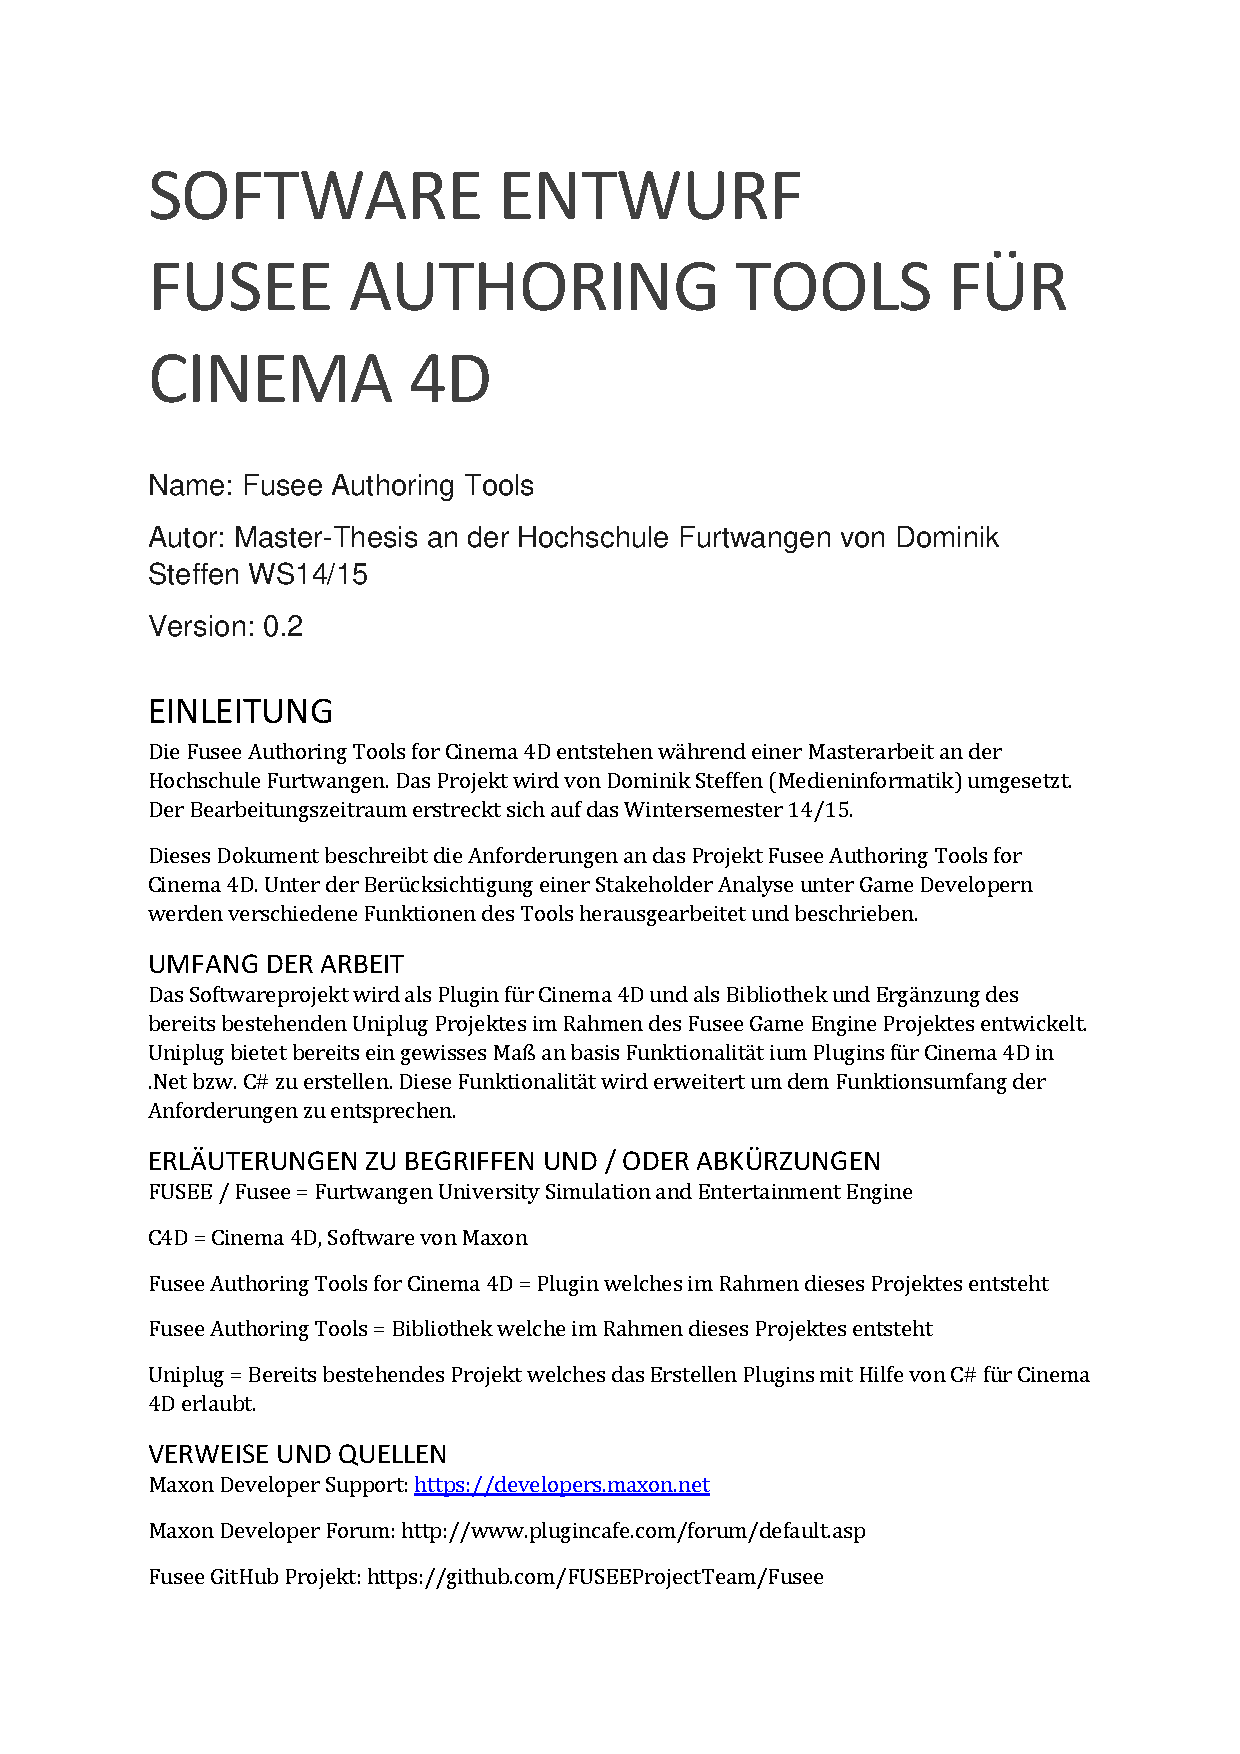
\includepdf[pages = 1-4]{Includes/SoftwareRequirementsSpecification.pdf}
%%%%%%%%%%%%%%%%%%%%%%%%%%%%%%%%%%%%%%%%%%%%%%%%%%%%%%%%%%%%%%%%%%%%%%%%%%%%%%%%
% Requirements ENDE
%%%%%%%%%%%%%%%%%%%%%%%%%%%%%%%%%%%%%%%%%%%%%%%%%%%%%%%%%%%%%%%%%%%%%%%%%%%%%%%%

%%%%%%%%%%%%%%%%%%%%%%%%%%%%%%%%%%%%%%%%%%%%%%%%%%%%%%%%%%%%%%%%%%%%%%%%%%%%%%%%
% UML START
%%%%%%%%%%%%%%%%%%%%%%%%%%%%%%%%%%%%%%%%%%%%%%%%%%%%%%%%%%%%%%%%%%%%%%%%%%%%%%%%
\chapter*{UML Diagramme}
\addcontentsline{toc}{chapter}{UML Diagramme}
%%%%%%%%%%%%%%%%%%%%%%%%%%%%%%%%%%%%%%%%%%%%%%%%%%%%%%%%%%%%%%%%%%%%%%%%%%%%%%%%
% UML ENDE
%%%%%%%%%%%%%%%%%%%%%%%%%%%%%%%%%%%%%%%%%%%%%%%%%%%%%%%%%%%%%%%%%%%%%%%%%%%%%%%%

%%%%%%%%%%%%%%%%%%%%%%%%%%%%%%%%%%%%%%%%%%%%%%%%%%%%%%%%%%%%%%%%%%%%%%%%%%%%%%%%
% Bilbiographie START
%%%%%%%%%%%%%%%%%%%%%%%%%%%%%%%%%%%%%%%%%%%%%%%%%%%%%%%%%%%%%%%%%%%%%%%%%%%%%%%%
\nocite{*}
\addcontentsline{toc}{chapter}{Literaturverzeichnis}
\printbibliography
\newpage
%%%%%%%%%%%%%%%%%%%%%%%%%%%%%%%%%%%%%%%%%%%%%%%%%%%%%%%%%%%%%%%%%%%%%%%%%%%%%%%%
% Bilbiographie ENDE
%%%%%%%%%%%%%%%%%%%%%%%%%%%%%%%%%%%%%%%%%%%%%%%%%%%%%%%%%%%%%%%%%%%%%%%%%%%%%%%%


\end{document}
